\section{Overview}
 
% main topic sentence for each paragraph

% 우리는 코드 변환을 기반을 기존의 모델을 자동으로 분산화하는 기법을 제안한다.
We propose the code transformation-based approach 
for automated distributed training of TensorFlow DL models.
As explained in the previous section, distributing TensorFlow DL models
with Horovod library requires adding and editing the origianl codes.
Currently, the developers must fully understand the model codes and
manually rewrite them.
This also includes understanding the Horovod library usage by reading
the library documentation and code exmaples.
To ease the burden of the rewriting process, 
we utilize the code transformation technique to automatically rewrite the
input TensorFlow model code with Horovod library.

% 기존의 모델에 적용하는 코드 변환 규칙을 정의하기 위해 horovod 라이브러리 문서와
% 코드 예제를 검토했다. 그 결과로 TF 모델을 4가지로 분류하고 각 분류에 맞는
% 변환 규칙을 정의할 수 있었다.
To define the code transformation rule for TensorFlow DL models,
we manually inspected the Horovod library documentation and code examples.
In this end, we identified four categories of TensorFlow DL models.
We define four \textit{training API patterns}, which are common code patterns of 
TensorFlow APIs appearing in each category of the TensorFlow DL models.
To categorize the TensorFlow DL models into one of the four patterns, 
we implemented the training API pattern identifier. 
In this process, we identified that the training API pattern identifier 
must know the class inheritance relationship between TensorFlow library 
classes and user-defined classes.
To solve this problem, we also implemented the class hierarchy analyzer to
retrieve the class inheritance information of the TensorFlow DL model.

\begin{figure}[ht!]
  \centering
  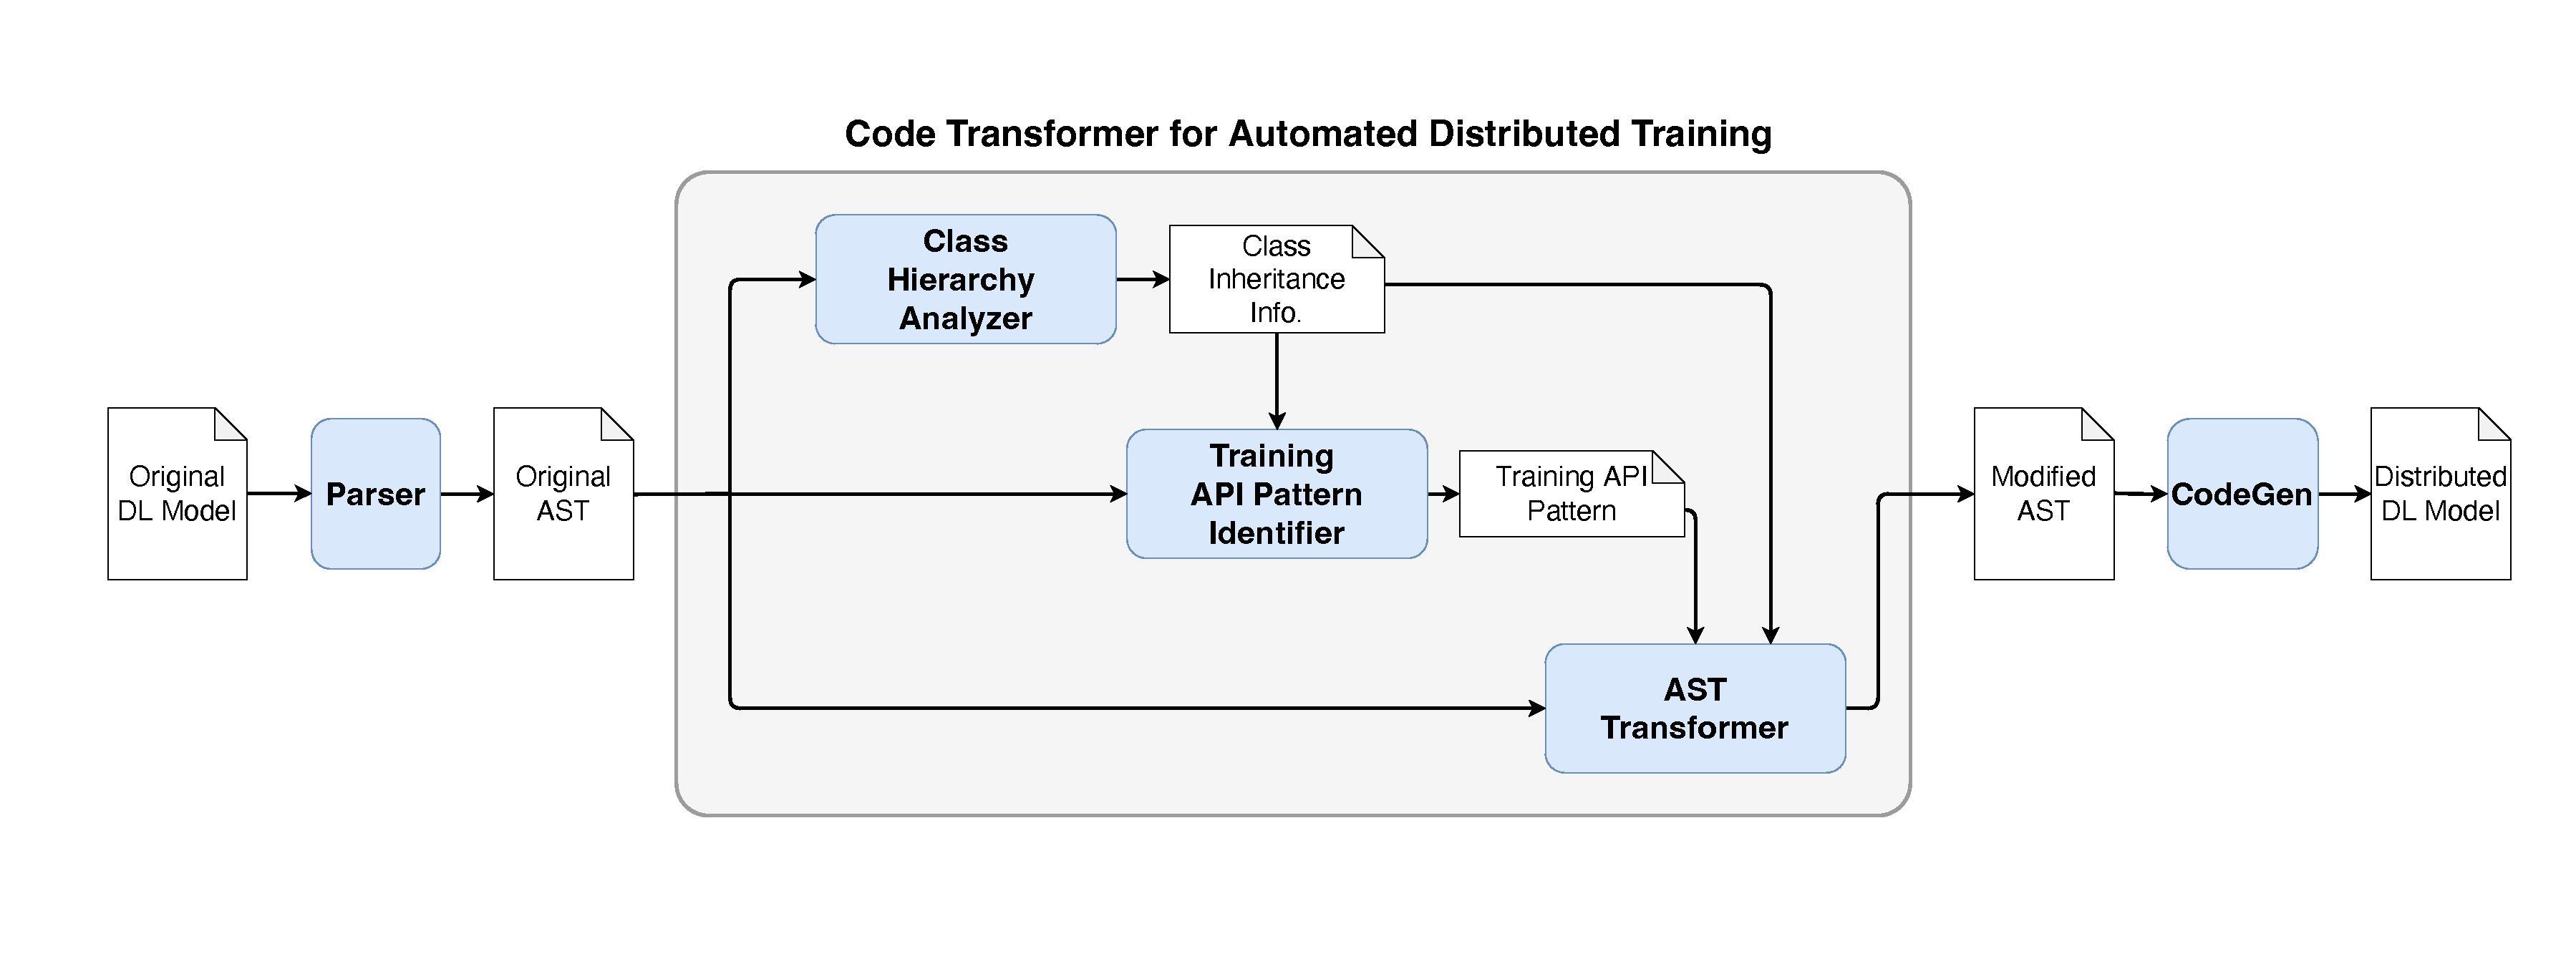
\includegraphics[width=\textwidth]{overview_diagram.pdf}
  \caption{Overall structure of the 
  automated transformation for distributed training}
  \label{sysarch}
\end{figure}

% 우리 기법은 입력으로 주어진 TF 모델에서 먼저 API 패턴을 인식하고
% 해당 패턴에 맞는 코드 변환 규칙을 적용하는 방식으로 작동한다.
% 이를 위해 설계한 우리 기법의 overview는 피규어와 같다...
Figure \ref{sysarch} illustrates the overview of our appraoch.
We first analyze the class hierarchy of the input TensorFlow model
to produce the class inheritance information.
Then the training API pattern identifier uses the inheritance information to
identify the training API pattern of the input model.
Finally, the AST transformer selects the correct transformation rule
according to the training API pattern then apply the rule to get the 
distributed model as an output.

\textbf{Parser}
Parser parses the input TensorFlow model codes into the ASTs.
We assume that the input model is given as a Python code
package in a single file directory.
Given the directory, the parser module first parses all Python code files
in the package to ASTs.
The section~\ref{sec:pysyn} describes the Python abstract syntax.

\textbf{Class Hierarchy Analyzer}
Class hierarchy analyzer analyzes the class inheritance relationship
between user-defined classes and TensorFlow library classes.
The class hierarchy analyzer produces the class hierarchy graph
which summarizes the class inheritance relationship of the input model.
The section~\ref{sec:cha} descrbies the details of the class hierarchy analyzer.

\textbf{Training API Pattern Identifier}
Training API pattern identifier uses the model AST and class inheritance 
information to recognize the TensorFlow APIs used in the training code and 
idenfity the training API pattern for the model.
The section~\ref{sec:pattern} describes the details of the training API pattern
identifier.

\textbf{AST Transformer}
AST transformer module applies the correct transformation to the
input model AST to produce the distributed training model AST.
To select the correct transformation rule,
the AST transformer utlizes the class inheritance information and
the training API pattern information.
We define the formal transformation rules which are composed of
the transform functions from ASTs to ASTs.
By applying the transform function to the input model AST,
the AST transformer produces the transformed AST as an output.
The section~\ref{sec:trans} describes the detailes of the AST transformer.
